%%%%%%%%%%%%%%%%%%%%%%%%%%%%%%%%%%%%%
%                                   %
% Compile with XeLaTeX and biber    %
%                                   %
% Questions or comments:            %
%                                   %
% joshua dot mcneill at uga dot edu %
%                                   %
%%%%%%%%%%%%%%%%%%%%%%%%%%%%%%%%%%%%%

\documentclass{beamer}
  % Read in standard preamble (cosmetic stuff)
  %%%%%%%%%%%%%%%%%%%%%%%%%%%%%%%%%%%%%%%%%%%%%%%%%%%%%%%%%%%%%%%%
% This is a standard preamble used in for all slide documents. %
% It basically contains cosmetic settings.                     %
%                                                              %
% Joshua McNeill                                               %
% joshua dot mcneill at uga dot edu                            %
%%%%%%%%%%%%%%%%%%%%%%%%%%%%%%%%%%%%%%%%%%%%%%%%%%%%%%%%%%%%%%%%

% Beamer settings
% \usetheme{Berkeley}
\usetheme{CambridgeUS}
% \usecolortheme{dove}
% \usecolortheme{rose}
\usecolortheme{seagull}
\usefonttheme{professionalfonts}
\usefonttheme{serif}
\setbeamertemplate{bibliography item}{}

% Packages and settings
\usepackage{fontspec}
  \setmainfont{Charis SIL}
\usepackage{hyperref}
  \hypersetup{colorlinks=true,
              allcolors=blue}
\usepackage{graphicx}
  \graphicspath{{../../figures/}}
\usepackage[normalem]{ulem}
\usepackage{enumerate}

% Document information
\author{M. McNeill}
\title[FREN2001]{Français 2001}
\institute{\url{joshua.mcneill@uga.edu}}
\date{}

%% Custom commands
% Lexical items
\newcommand{\lexi}[1]{\textit{#1}}
% Gloss
\newcommand{\gloss}[1]{`#1'}
\newcommand{\tinygloss}[1]{{\tiny`#1'}}
% Orthographic representations
\newcommand{\orth}[1]{$\langle$#1$\rangle$}
% Utterances (pragmatics)
\newcommand{\uttr}[1]{`#1'}
% Sentences (pragmatics)
\newcommand{\sent}[1]{\textit{#1}}
% Base dir for definitions
\newcommand{\defs}{../definitions}


  % Document information
  \subtitle[Computational Linguistics and Corpora]{Computational Linguistics and Corpora}

  %% Custom commands
  % Subsection/frame title
  \newcommand{\suboneone}{What is it?}
  \newcommand{\subtwoone}{}

\begin{document}
  % Read in the standard intro slides (title page and table of contents)
  %%%%%%%%%%%%%%%%%%%%%%%%%%%%%%%%%%%%%%%%%%%%%%%%%%%%%%%%%%%%%%%%
% This is a standard set of intro slides used in for all slide %
% documents. It basically contains the title page and table of %
% contents.                                                    %
%                                                              %
% Joshua McNeill                                               %
% joshua dot mcneill at uga dot edu                            %
%%%%%%%%%%%%%%%%%%%%%%%%%%%%%%%%%%%%%%%%%%%%%%%%%%%%%%%%%%%%%%%%

\begin{frame}
  \titlepage
  \tiny{Office: % Basically a variable for office hours location
Gilbert 121\\
        Office hours: % Basically a variable for office hours
 lundi, mercredi, vendredi 10:10--11:10
}
\end{frame}

\begin{frame}
  \tableofcontents[hideallsubsections]
\end{frame}

\AtBeginSection[]{
  \begin{frame}
    \tableofcontents[currentsection,
                     hideallsubsections]
  \end{frame}
}


  \section{Computational Linguistics and Corpora}
    \subsection{\suboneone}
      \begin{frame}{\suboneone}
        \begin{definition}
          % Computational linguistics
The study of how to engineer computers to process and produce language

          \only<1>{
            \begin{itemize}
              \item Also called \alert{natural language processing}
            \end{itemize}
          }
        \end{definition}
        \begin{block}{Two goals of this engineering}
          \only<1>{
            Basing models on linguistic theories allows us to test those theories
          }
          \only<2->{
            Models allow us to interact with computers and process data more efficiently
          }
        \end{block}
        \uncover<2->{
          \begin{columns}
            \column{0.5\linewidth}
              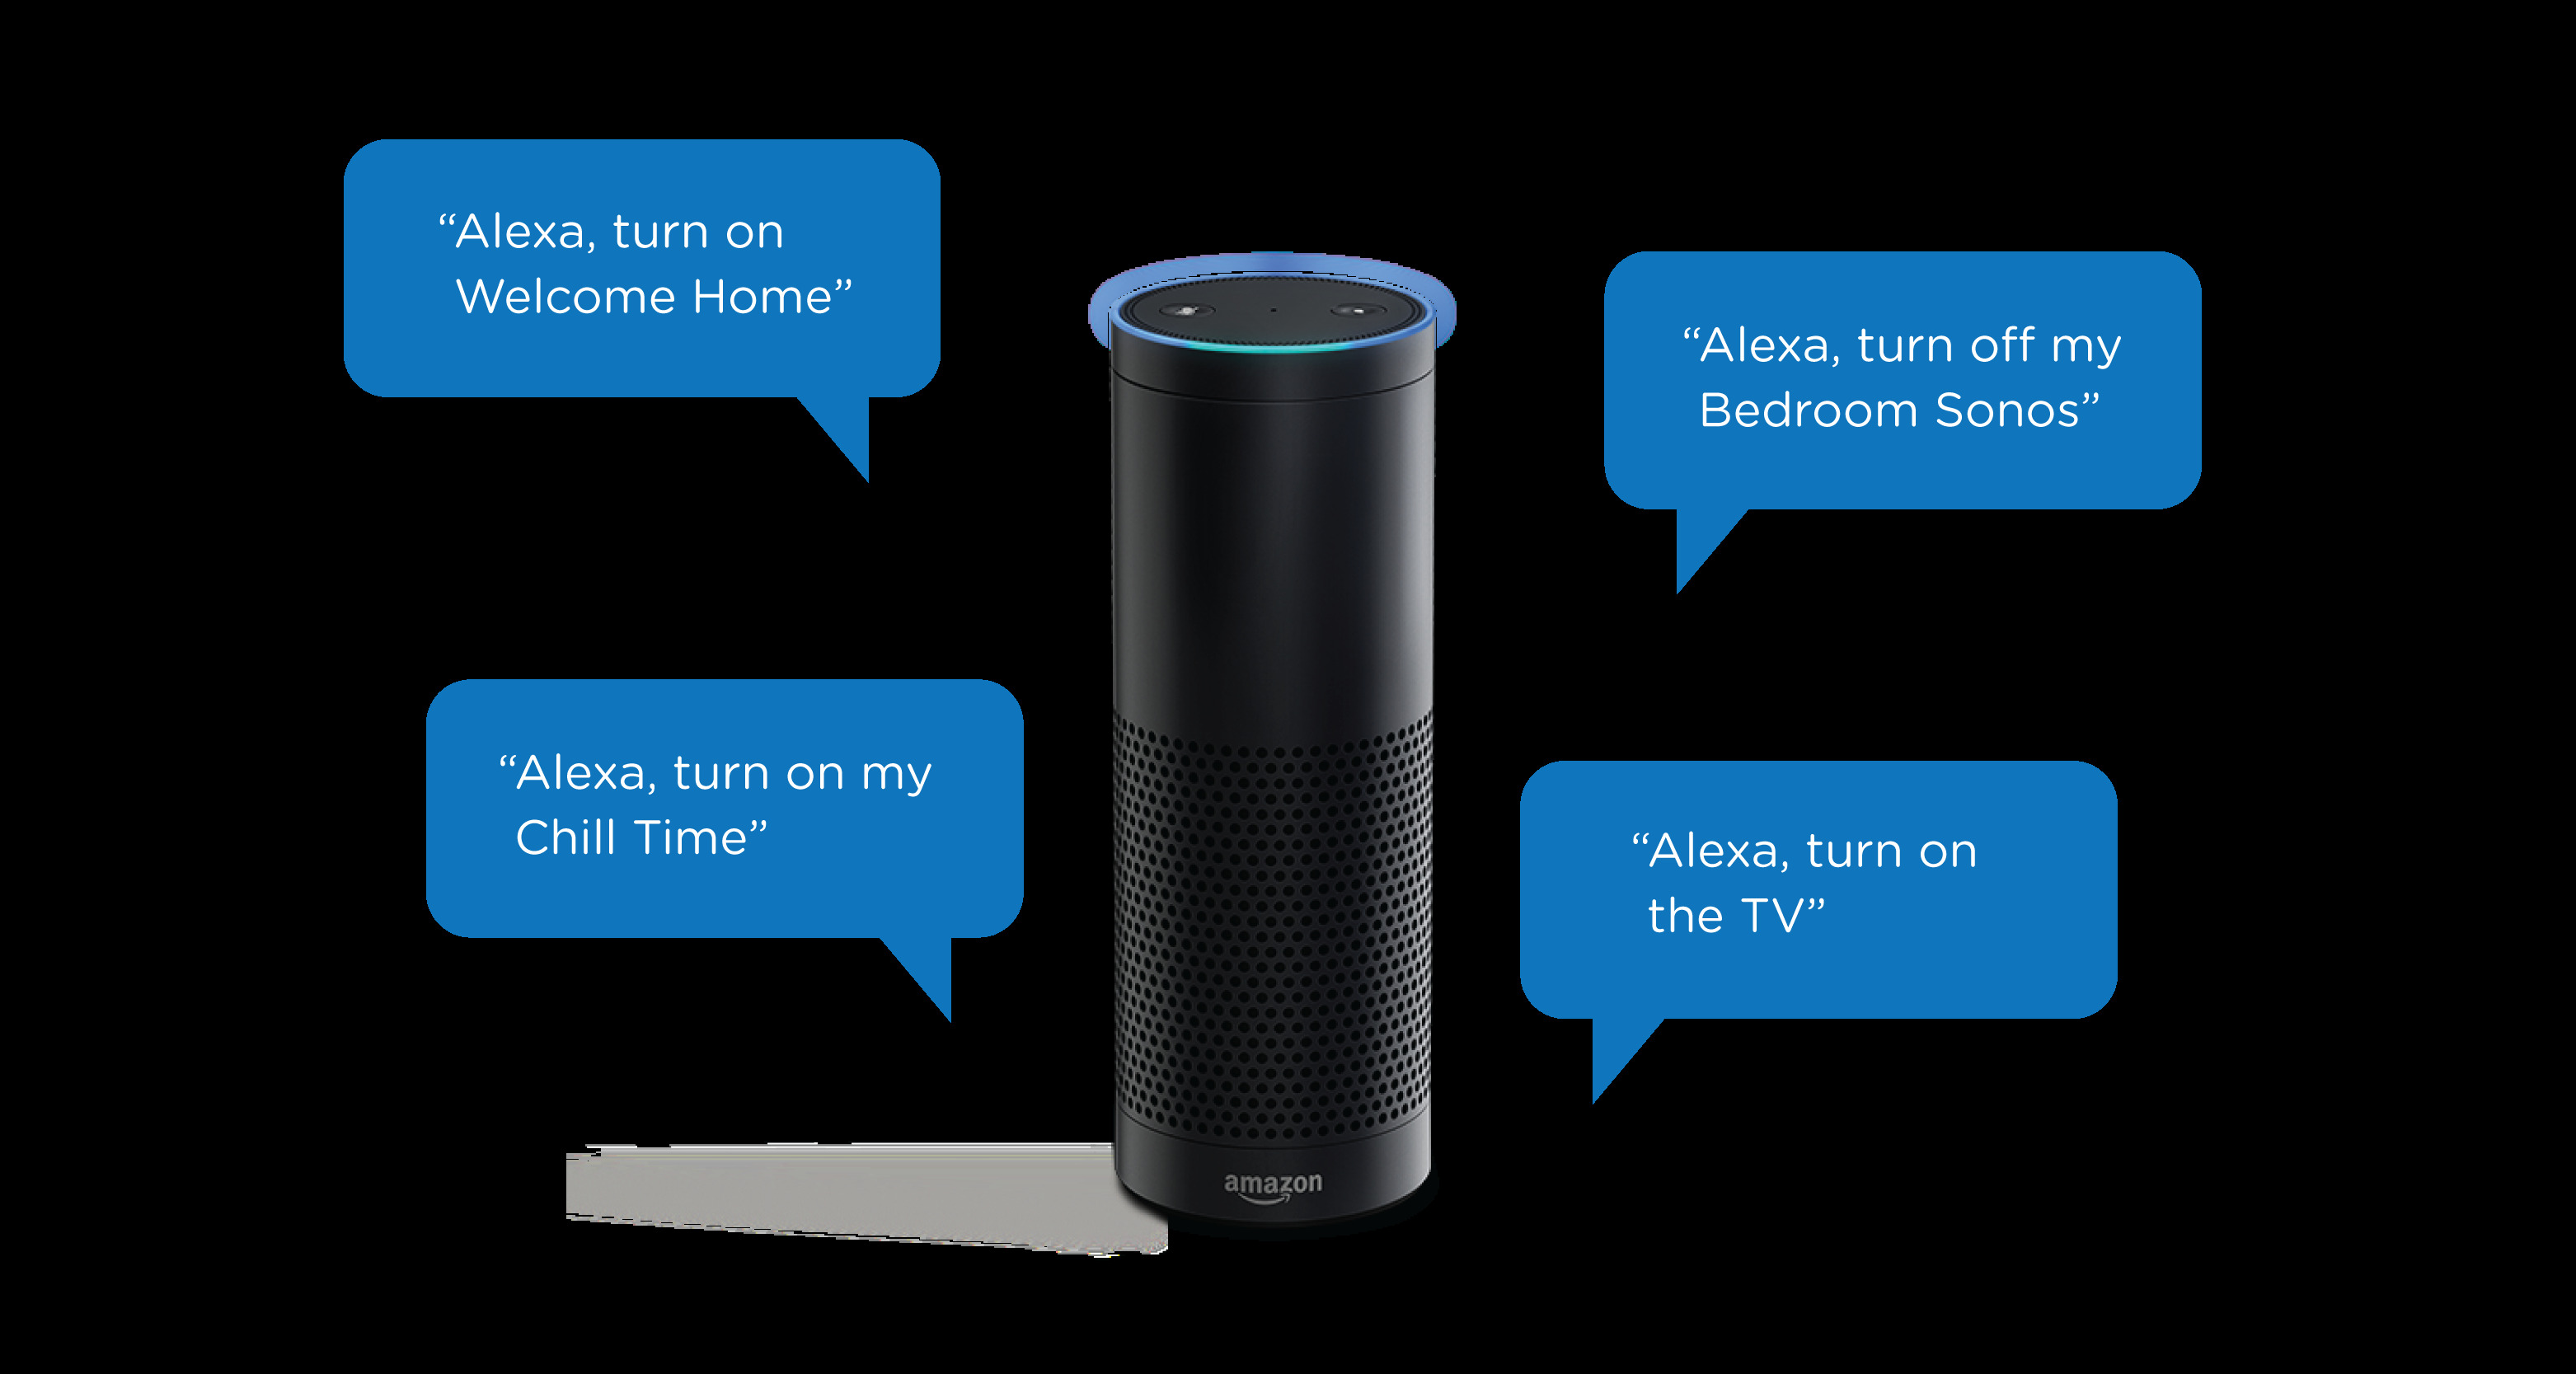
\includegraphics[scale=0.1]{alexa.jpg}
            \column{0.5\linewidth}
              
\includegraphics[scale=0.325]{autocomplete_dino.jpg}
          \end{columns}
        }
      \end{frame}

  \section{Corpora}
    \subsection{\subtwoone}
      \begin{frame}{\subtwoone}

      \end{frame}

    \subsection{}
      \begin{frame}{}
        \begin{block}{Try these}
          % \textcite{dawson_language_2016}, chapter 16 exercises
        \end{block}
      \end{frame}

      \begin{frame}{References}
        % \printbibliography
      \end{frame}
\end{document}
